\documentclass[a4paper,12pt]{article}

\usepackage{graphicx}
\usepackage{hyperref}
\graphicspath{{images/}}
\begin{document}

\section{Use Case: Summarize Thread}
This use case deals with the service of summarizing threads. A user will be able to summarize a thread once he/she has gained the required level. The original tread will then be replaced with the summarized one. The original thread will not be removed, instead it will be hidden from view of users.
    
    
\subsection{Use Case Prioritization}
This feature of the forum is not a critical one. This is an added benefit to the administrators and the users to simplify the viewing of important posts on a long enough thread.
      
\subsection{Service Contracts}
Pre-conditions: 
\begin{itemize}
\item The user must be registered(no guest accounts/spectators)
\item The user must have this privilege
\item The database must be online
\item The database must be connected
\item The thread must be long enough to warrant a summary
\end{itemize}
      
Post-Conditions:
\begin{itemize}
\item The changes must reflect in the database
\item The original thread must be hidden
\item The summarized thread should now be visible
\end{itemize}
      
\subsection{Process}
A user, that has the required privileges, will request a summary to be made of a thread. The thread(link??) is then used passed as a parameter to the function/object that will facilitate the summarizing. First a check for the users status will be done to see whether this request is allowed. If the request is not refused then a call to the database is made requesting the tread. A new thread will also be made to store the new summary. An algorithm that takes into account the original poster, the poster with the best solution and posts that have the highest votes will be used to make the summary. The original thread will then be made invisible to users while the summarized thread will replace it. The new thread will also be stored in the database.

\subsection{Use Case Diagram}
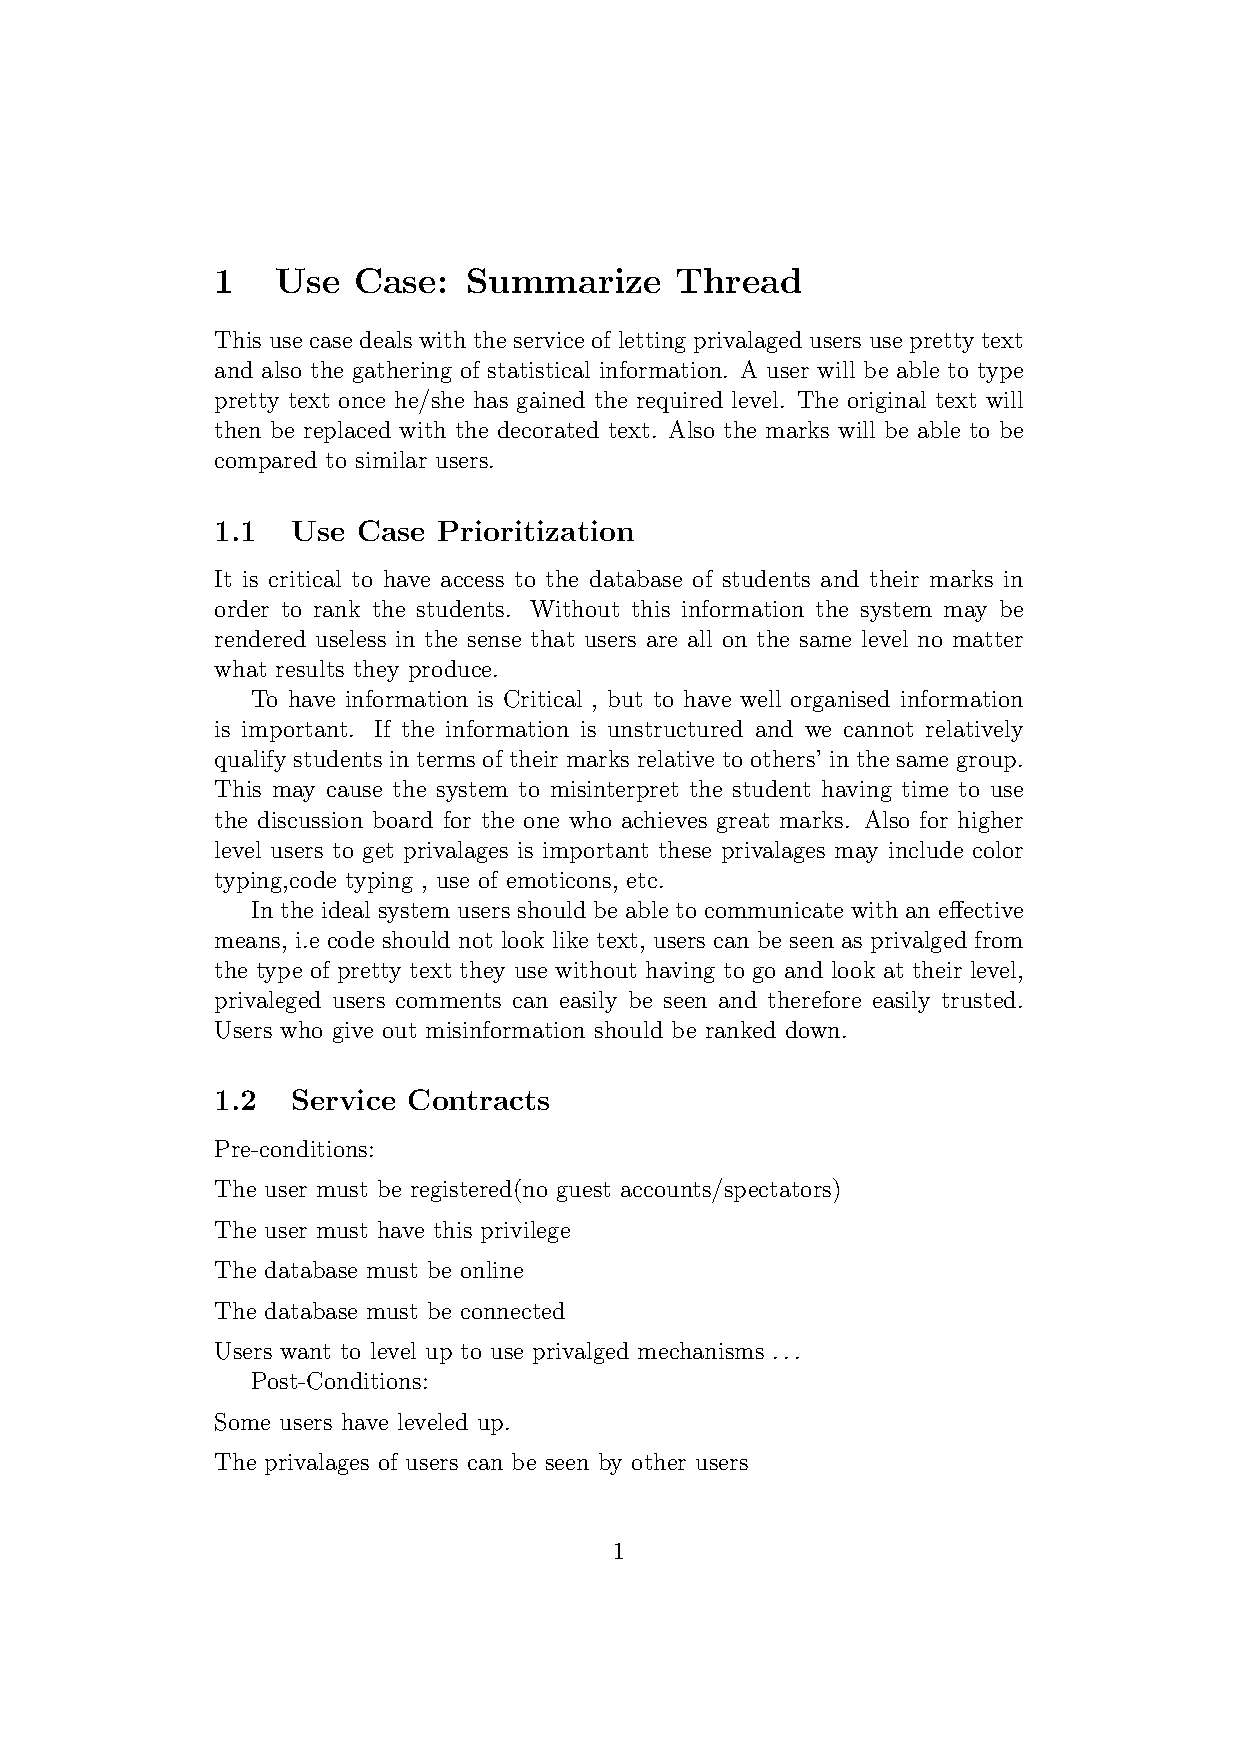
\includegraphics{12260429_SummarizeThread}

\end{document}
